%================================
\subsection{Resultados algoritmo secuencial}
\label{sec:Resultados algoritmo secuencial}

Estos son los resultados de cada una de las versiones secuenciales, implementadas para el Reto 2, ejecutadas en una de las maquinas de AWS antes descritas.

\begin{table}[H]
    \centering
    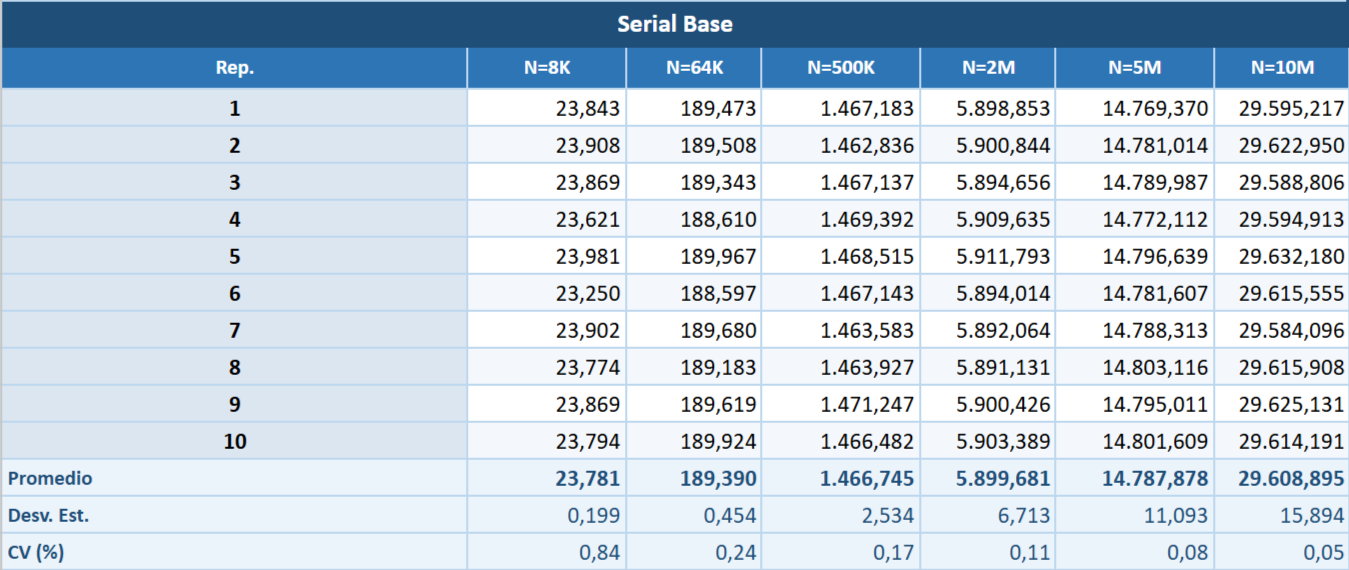
\includegraphics[width=1\textwidth]{images/tables/time_secuencial_noopt.png}
    \caption{Tiempos de ejecución del algoritmo secuencial sin optimizaciones}
\end{table}

\begin{table}[H]
    \centering
    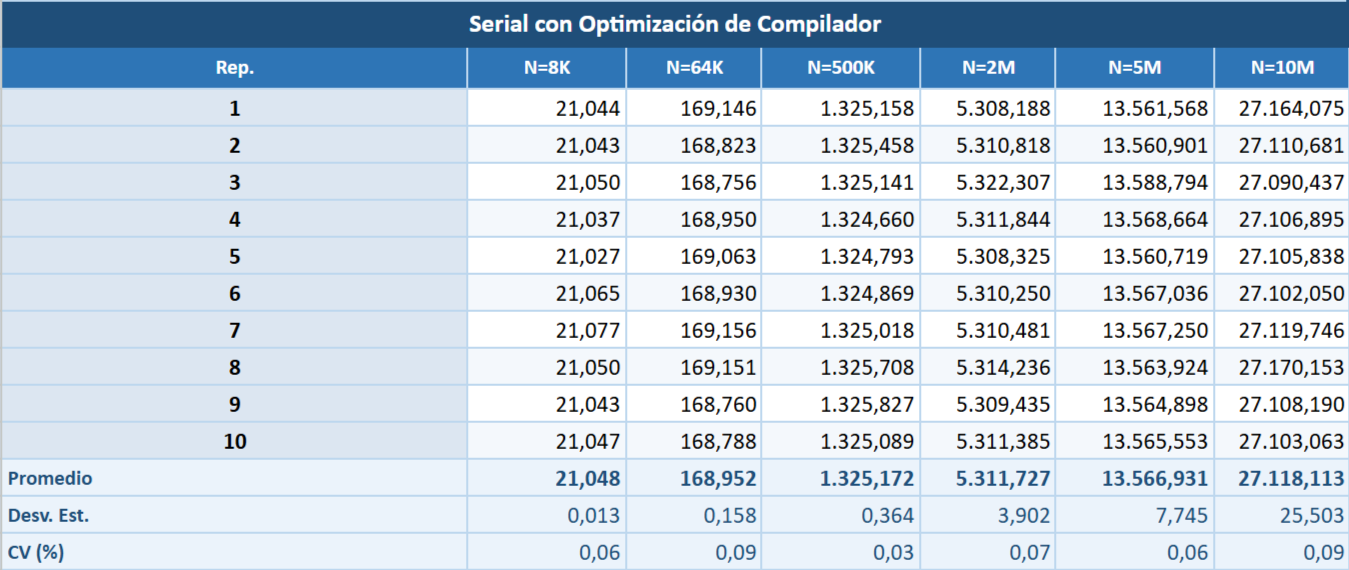
\includegraphics[width=1\textwidth]{images/tables/time_secuencial_opt.png}
    \caption{Tiempos de ejecución del algoritmo secuencial con optimización por compilador}
\end{table}

\begin{table}[H]
    \centering
    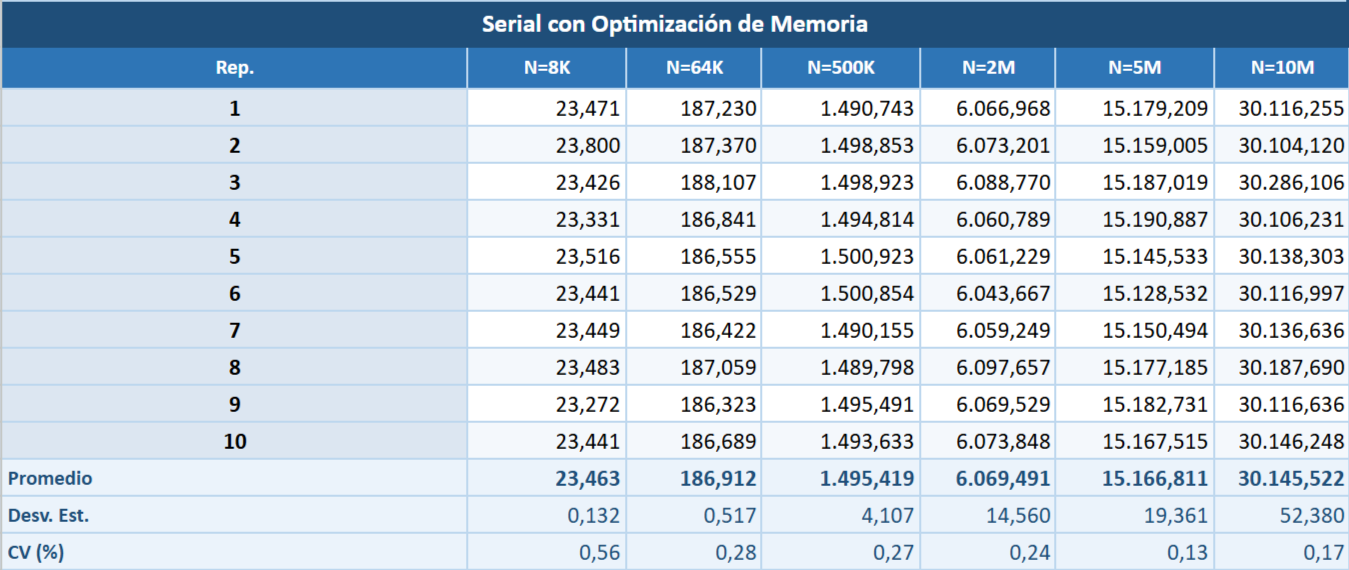
\includegraphics[width=1\textwidth]{images/tables/time_secuencial_mem.png}
    \caption{Tiempos de ejecución del algoritmo secuencial con optimización por memoria}
\end{table}

\begin{table}[H]
    \centering
    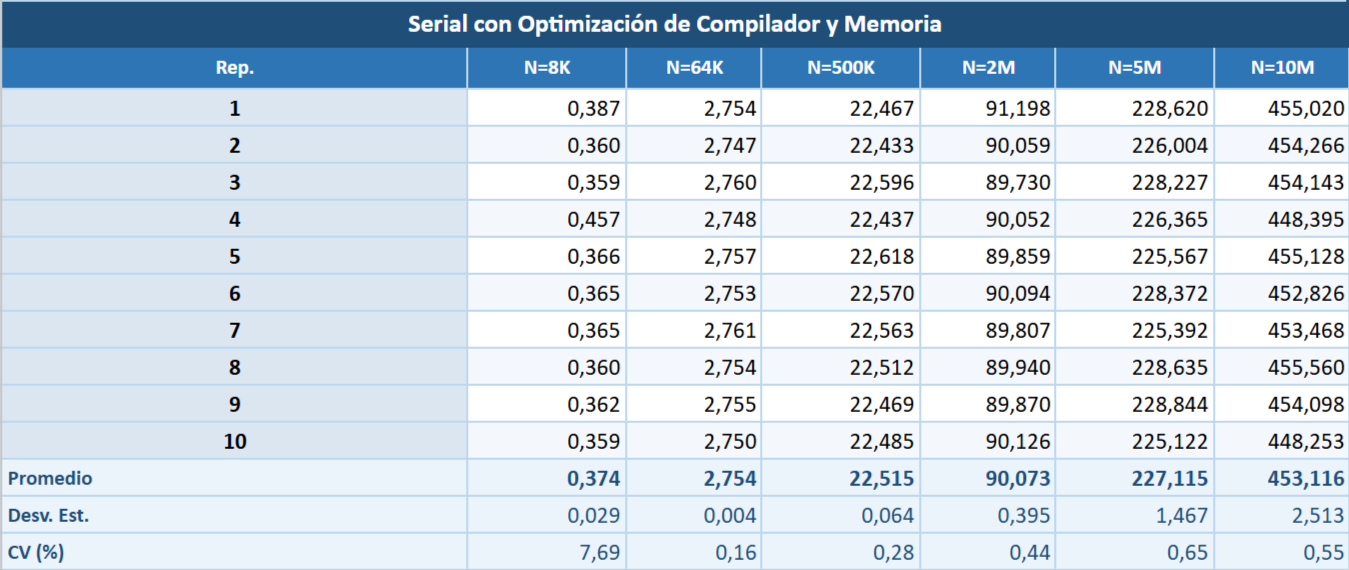
\includegraphics[width=1\textwidth]{images/tables/time_secuencial_mem_opt.png}
    \caption{Tiempos de ejecución del algoritmo secuencial con optimización por compilador y memoria}
\end{table}

\begin{figure}[H]
   \centering
   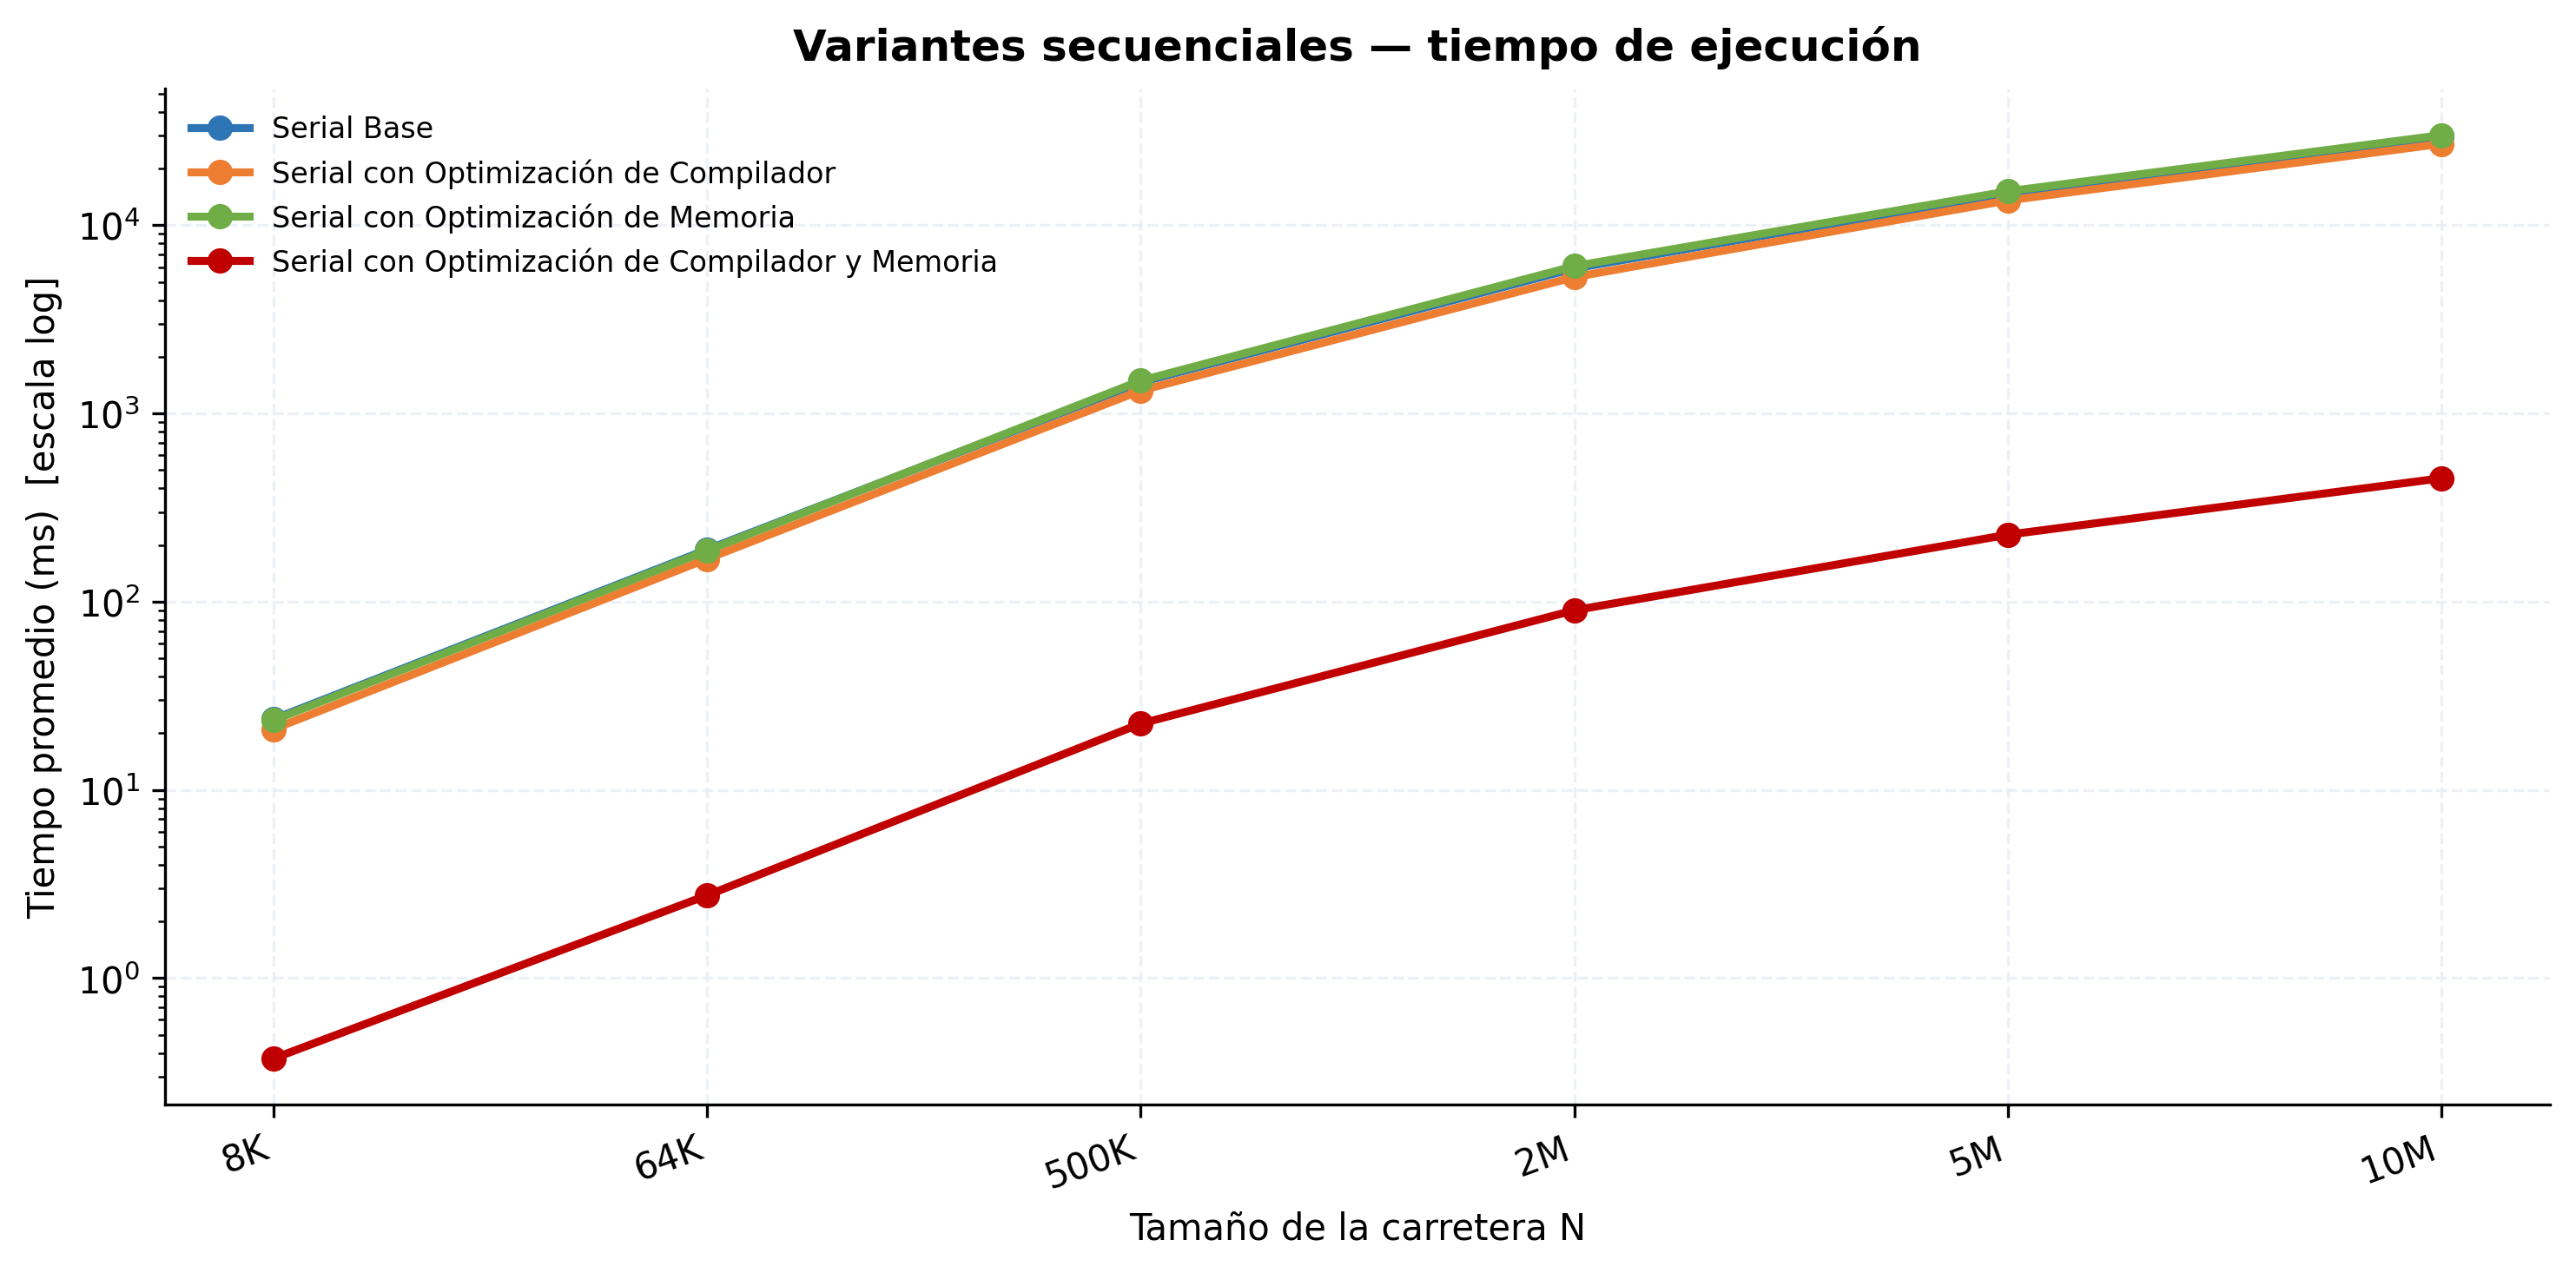
\includegraphics[width=1\textwidth]{images/charts/time_secuencial.png}
   \caption{Gráfica de tiempos de los algoritmos secuenciales}
\end{figure}

\begin{table}[H]
    \centering
    
\includegraphics[width=1\textwidth]{images/tables/speedup_secuencial.png}
    \caption{Speedup de las versiones secuenciales}
\end{table}

\begin{figure}[H]
   \centering
   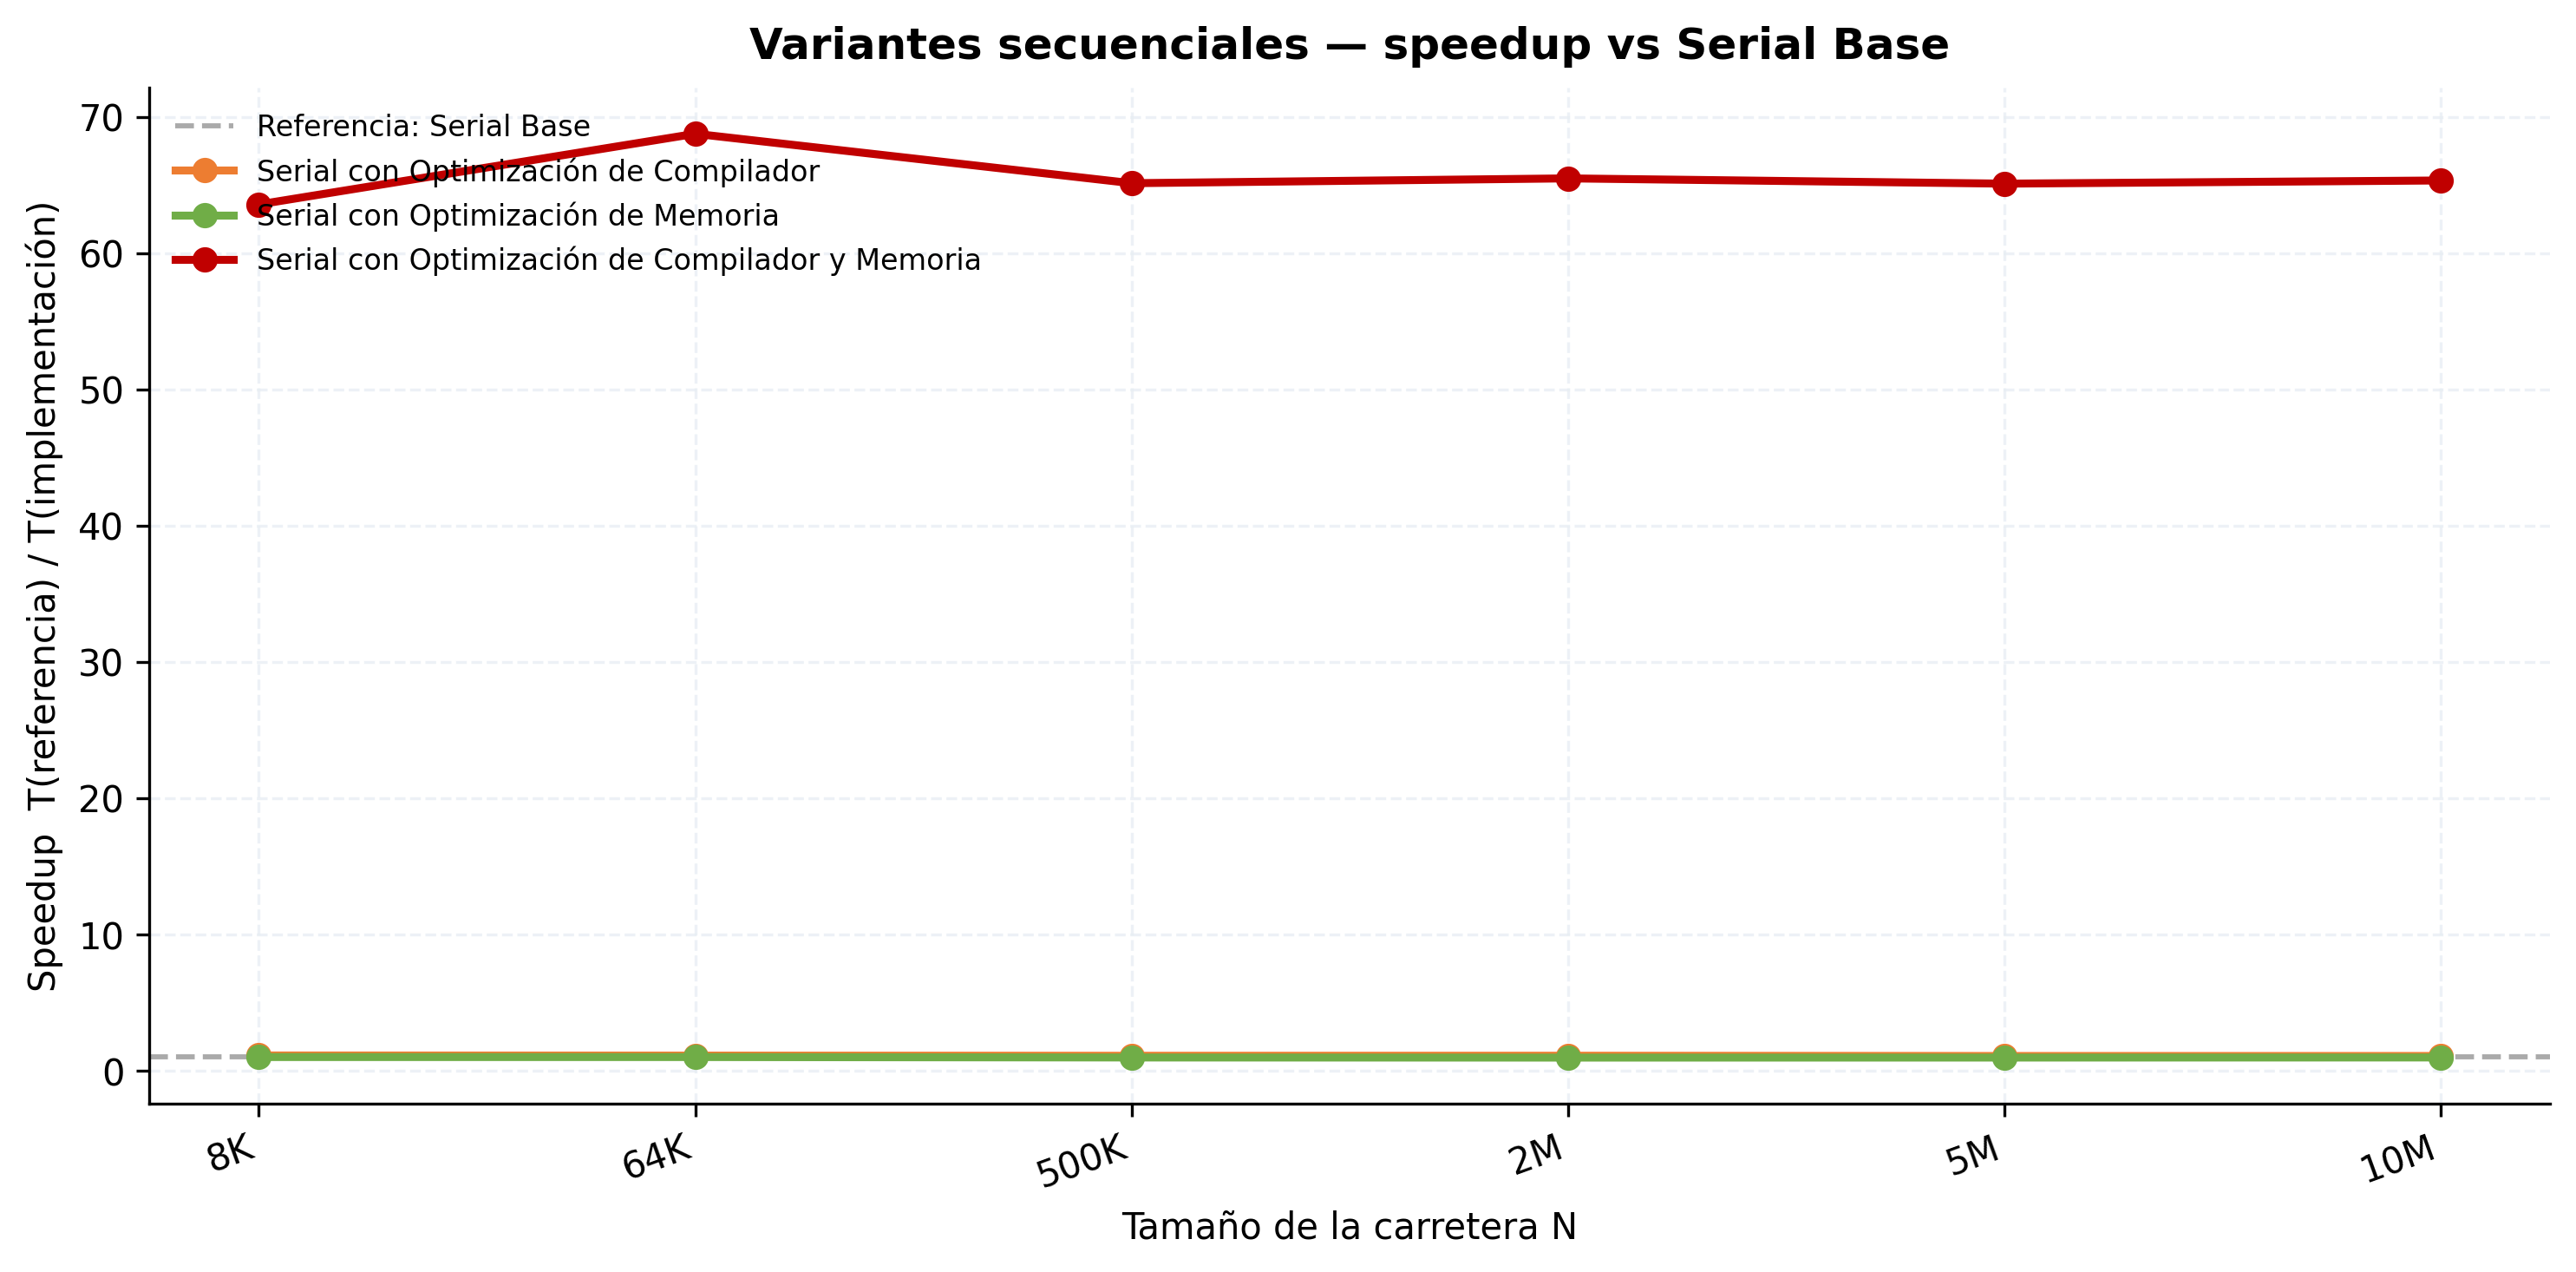
\includegraphics[width=1\textwidth]{images/charts/speedup_secuencial.png}
   \caption{Gráfica de Speedup de los algoritmos secuenciales}
\end{figure}